\documentclass[math, english, info]{beamercours}
\makeatletter
\def\tikzimp@rt{1}
\makeatother

\bibliography{tdparse.bib}

\usepackage{bigstrut}
\usepackage{makecell}
\usepackage{emoji}
\usepackage{tikz-dependency}
\usepackage{diag}

\def\cont{\Gamma\vdash}
\def\poulpe{\qquad}

\setlength\belowcaptionskip{0pt}
\setlength\abovecaptionskip{\baselineskip}

\DeclareMathOperator{\Var}{Var}

\def\ppl{\mathbin{+\mkern-12mu+}}

\makeatletter
\renewenvironment{thebibliography}[1]
     {\section{\bibname}
      \@mkboth{\MakeUppercase\bibname}{\MakeUppercase\bibname}%
      \list{\@biblabel{\@arabic\c@enumiv}}%
           {\settowidth\labelwidth{\@biblabel{#1}}%
            \leftmargin\labelwidth
            \advance\leftmargin\labelsep
            \@openbib@code
            \usecounter{enumiv}%
            \let\p@enumiv\@empty
            \renewcommand\theenumiv{\@arabic\c@enumiv}}%
      \sloppy
      \clubpenalty4000
      \@clubpenalty \clubpenalty
      \widowpenalty4000%
      \sfcode`\.\@m}
     {\def\@noitemerr
       {\@latex@warning{Empty `thebibliography' environment}}%
      \endlist}

\def\black@or@white#1#2{%
  \@tempdima#2 pt
  \ifdim\@tempdima>0.5 pt
    \definecolor{temp@c}{gray}{0}%
  \else
    \definecolor{temp@c}{gray}{1}%
  \fi}
\def\letterbox#1#{\protect\letterb@x{#1}}
\def\letterb@x#1#2#3{%
  \colorlet{temp@c}[gray]{#2}%
  \extractcolorspec{temp@c}{\color@spec}%
  \expandafter\black@or@white\color@spec
  {\color#1{temp@c}\tallcbox#1{#2}{#3}}}
\def\tallcbox#1#{\protect\color@box{#1}}
\def\color@box#1#2{\color@b@x\relax{\color#1{#2}}}
\long\def\color@b@x#1#2#3%
 {\leavevmode
  \setbox\z@\hbox{{\set@color#3}}%
  \ht\z@\ht\strutbox
  \dp\z@\dp\strutbox
  {#1{#2\color@block{\wd\z@}{\ht\z@}{\dp\z@}\box\z@}}}
\makeatother

\contourlength{0.005em}
\def\backbox#1{\letterbox{Lavender!40}{\contour{black}{#1}}}

\def\ty#1{\backbox{\tt\color{yulm!90!black}#1}}
\def\f#1{\backbox{\tt\color{vulm}#1}}
\def\w#1{\mathbf{#1}\,}

\def\e{\ty{e}}
\def\t{\ty{t}}
\def\r{\ty{r}}

\newcolumntype{C}{>{$}c<{$}}
\newcolumntype{L}{>{$}l<{$}}
\newcolumntype{R}{>{$}r<{$}}
\def\fmap{\texttt{fmap}}


\makeatletter
\newcommand{\@word}[4][]{%
	#2 & #3 & #4\\
\ifx&#1&%
	%
\else
	&\multicolumn{2}{l}{Generalizes to \textbf{#1}}\\%
\fi%
}
\def\word#1#2#3#4{\@word[#4]{#1}{#2}{#3}}
\makeatother

\usepackage{calc}

\makeatletter
\def\textSq#1{%
\begingroup% make boxes and lengths local
\setlength{\fboxsep}{0.4ex}% SET ANY DESIRED PADDING HERE
\setbox1=\hbox{#1}% save the contents
\setlength{\@tempdima}{\maxof{\wd1}{\ht1+\dp1}}% size of the box
\setlength{\@tempdimb}{(\@tempdima-\ht1+\dp1)/2}% vertical raise
\raise-\@tempdimb\hbox{\fbox{\vbox to \@tempdima{%
  \vfil\hbox to \@tempdima{\hfil\copy1\hfil}\vfil}}}%
\endgroup%
}
\def\Sq#1{\textSq{\ensuremath{#1}}}%

\def\c@lsep{2.3}
\def\r@wsep{.8}

\tikzset{
	uptree/.style={
			draw=green!80!black,
			thick,
		},
	typenode/.style={
			align=center,
			text width=24mm,
			%font={\large},
		},
	treenode/.style={
			align=center,
			text width=24mm,
		},
	wordnode/.style={
			inner sep=0pt,
			align=center,
			font={\large},
		},
	downtree/.style={
			draw=red!80!black,
			thick,
		},
}

\newcommand{\wnode}[3]{%
	\node (#2) at (#1*\c@lsep, 0) [wordnode] {#2};
	\node[anchor=north] (#2-) at ($(#1*\c@lsep, 0) + (0, -.142)$) [typenode] {\ensuremath{#3}};
}
\newcommand{\utnode}[3]{%
	\path let \p1 = (#2.north), \p2 = (#3.north) in coordinate (Q1) at (\x1, {max(\y1, \y2)});
	\path let \p1 = (#2.north), \p2 = (#3.north) in coordinate (Q2) at (\x2, {max(\y1, \y2)});
	\node (#2#3) at ($($(Q1)!0.5!(Q2)$) + (0, 1)$) [treenode] {\ensuremath{#1}};
	\draw[uptree] ($(#2.north) + (0, .142)$) -- (#2#3.south);
	\draw[uptree] ($(#3.north) + (0, .142)$) -- (#2#3.south);
}
\newcommand{\dtnode}[4][0.5]{%
	\path let \p1 = (#3.south), \p2 = (#4.south) in coordinate (Q1) at (\x1, {min(\y1, \y2)});
	\path let \p1 = (#3.south), \p2 = (#4.south) in coordinate (Q2) at (\x2, {min(\y1, \y2)});
	\node (#3#4) at ($($(Q1)!#1!(Q2)$) + (0, -1)$) [treenode] {\ensuremath{#2}};
	\draw[downtree] ($(#3.south) + (0, -.142)$) -- (#3#4.north);
	\draw[downtree] ($(#4.south) + (0, -.142)$) -- (#3#4.north);
}

\def\inputtikz#1{
	\ifnum\tikzimp@rt=1
		\input{figures/#1}
	\else
		\ensuremath{\text{\Huge\color{vulm}A TikZ PICTURE GOES HERE.}}
	\fi
}
\makeatother

\catstyle{catone}{gray!50}
\catstyle{catmc}{vulm!10!yulm}
\catstyle{catmca}{vulm!20!yulm}
\catstyle{catmcb}{vulm!30!yulm}
\catstyle{catmcc}{vulm!40!yulm}
\catstyle{catmcd}{vulm!50!yulm}
\catstyle{catmce}{vulm!60!yulm}
\catstyle{catmcf}{vulm!70!yulm}
\catstyle{catmcg}{vulm!80!yulm}
\catstyle{catmch}{vulm!90!yulm}

\def\din#1{#1\mathrm{.S}}
\def\dnb#1{#1\mathrm{.N}}
\def\dlb#1#2{#1\mathrm{.L}\left(#2\right)}
\def\dl#1{#1\mathrm{.L}}
\def\dnlg#1{#1\mathrm{.h}}
\def\dnin#1{#1\mathrm{.in}}
\def\dnout#1{#1\mathrm{.out}}

\newcounter{lingexcnt}
\newcounter{tmplingexcnt}
\renewcommand*{\thelingexcnt}{(\arabic{lingexcnt})}
\newenvironment{sentence}[1][]{
     \begin{list}{\thelingexcnt}{\refstepcounter{lingexcnt}}\item
     \ifnum\pdfstrcmp{#1}{}=0\else\label{#1}\fi
}{\end{list}}

\newenvironment{nsentence}{%
     \setcounter{tmplingexcnt}{\value{lingexcnt}}
     \addtocounter{tmplingexcnt}{-1}
     \begin{list}{\thelingexcnt}{
         \usecounter{lingexcnt}
         \setcounter{lingexcnt}{\value{tmplingexcnt}}
         \refstepcounter{lingexcnt}
     }
}{\end{list}}

\newcommand*{\oneSentence}[2][]{\begin{sentence}[#1]#2\end{sentence}}

\DeclareFieldFormat{urldate}{}

\title{Effect-Driven Parsing}
\subtitle{Formal studies on a categorical approach to semantic parsing}
\institute{École Normale Supérieure | Yale University}
\author{Matthieu Boyer}
\date{September 9 2025}
\addlogo{~/Pictures/Yale_University_logo.svg.png}
\addlogo{~/DEV/latex/source/ens_psl.pdf}

\begin{document}
\fancytitleframe

\section{Introduction}
\subsection{General Introduction}
\begin{frame}
	\frametitle{Context}
	\begin{itemize}
		\item Categorical formalization of a type and effects system for
		      natural-language semantics
		      (following \cite{bumfordEffectdrivenInterpretationFunctors2025}).

		\item Develop a graphical, type-driven parsing formalism that
		      derives sentence meaning compositionally from word meanings.
	\end{itemize}
\end{frame}

\begin{frame}[fragile]
	\frametitle{Typed Semantics for Natural Languages}
	\begin{center}
		\setcellgapes{3pt}
		\makegapedcells
		\begin{NiceTabular}{>{\bf}LLL}
			Expression & \rm Type & \lambda\text{-Term} \\
			\word{planet}{\e\to\t}{\lambda x. \w{planet} x}{common nouns}
			\word{Jupiter}{\e}{{\bf j}\in \Var}{proper nouns}
			\word{chase}{\e \to \e \to \t}{\lambda o. \lambda s. \mathbf{chase}\left( o \right)\left( s \right)}{transitive verbs}
			\CodeAfter
			\begin{tikzpicture}
				\draw[double] (1|-2) -- (4|-2);
				\foreach \r in {4,6} {\draw (1|-\r) -- (4|-\r);}
			\end{tikzpicture}
		\end{NiceTabular}
	\end{center}
\end{frame}

\begin{frame}[fragile]
	\frametitle{Syntactic Types and Semantic Types}
	\begin{itemize}
		\item Syntax \textbf{a cat} and \textbf{the cat} should have the same type: $\e$.
		      \pause
		\item No single canonical \textbf{cat} exists: that type cannot be $\e$.
	\end{itemize}
	\pause

	We will use \textbf{(side-)effects} to do the difference between them:
	\begin{equation*}
		\w{a\ cat} = \{c \mid \w{cat} c\} \tag{Set}
	\end{equation*}
	\begin{equation*}
		\w{the\ cat} = x \text{ if } \mathbf{cat}^{-1}(\top) = \{x\} \text{ else } \# \tag{Maybe}
	\end{equation*}
\end{frame}

\subsection{Categorical Introduction}
\begin{frame}
	\frametitle{Effects as Functors}
	Traditionally (\cite{moggiComputationalLambdacalculusMonads1989}), monads model side-effects.
	\pause

	Here, functors suffice and lighter structures are useful.
\end{frame}

\begin{frame}
	\frametitle{String Diagrams}
	String Diagrams are a formalism (\cite{hinzeIntroducingStringDiagrams2023})
	for visualising multi-threading computations.

	\medskip

	Theoretically, the dual of a diagram in a 2-category.

	\pause
	\medskip
	Used as a tool for parsing in \cite{coeckeMathematicalFoundationsCompositional2010}.
\end{frame}

\begin{frame}
	\frametitle{Other Categorical Theories}
	\cite{marcollimatildeetchomskynoametberwickrobertc.MathematicalStructureSyntactic}
	and \cite{senturiaAlgebraicStructureMorphosyntax2025} use Hopf algebras to
	give a model for parsing.

	\medskip

	\cite{melliesCategoricalContoursChomskySchutzenberger2025} use operads to
	prove results on CFGs.
\end{frame}

\section{Category-theoretical type system}
\subsection{Type system}
\begin{frame}
	\frametitle{Notations}
	\begin{itemize}
		\item Language $\mL$ of denotationally composed words.
		\item Base typing CCC $\mC$; Effects: functors $\mathcal{F}(\mL)$.
		      \pause
		\item Typing CCC: $\bar{\mC}$ = closure of $\mC$ under $\mathcal{F}(\mL)^{*}$, products and exponentials.
	\end{itemize}
	Intuition: all (effect-sequence, base type) combos, with functions/products.
\end{frame}

\begin{frame}[fragile]
	\frametitle{Intuitionistic-style Typing Judgements}
	\only<1-2>{We then have typing judgements for basic combinations:
		\begin{align*}
			\only<1>{
			\frac{\cont x: \tau \poulpe \cont F \in \mathcal{F}(\mL)}{\cont Fx: F\tau }\fracnotate{Cons}               \\[.25cm]
				\frac{\cont x: F\tau_{1} \poulpe \cont \phi: \tau_{1} \to \tau_{2}}{\cont \phi x: F\tau_{2} }\fracnotate{\texttt{fmap}}
			}
			\only<2>{
			\frac{\cont x: \tau_{1} \poulpe \cont \phi: \tau_{1} \to \tau_{2}}{\cont \phi x: \tau_{2}}\fracnotate{App} \\[.25cm]
				\frac{\cont x: A\tau_{1} \poulpe \cont \phi: A\left( \tau_{1} \to \tau_{2} \right)}{\cont \phi x: A\tau_{2}}\fracnotate{\texttt{<*>}}
			}
		\end{align*}
	}
	\only<3>{Typing judgements for natural transformations:
		\begin{align*}
			\frac{\cont x: \tau}{\cont x: A\tau}\fracnotate{\texttt{pure/return}} \\[.25cm]
			\frac{\cont x: MM\tau}{\cont x: M\tau}\fracnotate{\texttt{>>=}}
		\end{align*}
		\begin{align*}
			\forall F \overset{\theta}{\Longrightarrow} G,\poulpe \frac{\cont x: F\tau \poulpe \cont G: S' \subseteq \star \poulpe \tau \in S'}{\cont x : G\tau}\fracnotate{\texttt{nat}}
		\end{align*}
	}
\end{frame}

\subsection{Introducing a language}

\begin{frame}
	\frametitle{Presentation}
	To present a language in our formalism, we need:
	\begin{itemize}
		\item A syntax;
		\item A typed dictionary using effects;
		\item A typed lexicon of non-verbal constructs.
	\end{itemize}
\end{frame}

\begin{frame}
	\frametitle{Introducing Higher-Order Constructs}
	We implement higher-order semantics (e.g. the future and plural) via functors.

	\pause
	\smallskip

	We also enforce the notion of scope islands
	as in \cite{bumfordEffectdrivenInterpretationFunctors2025}:

	\begin{equation*}
		\w{if}: \left(\t \setminus \mF\left(\mL\right)^{*}\f{C}\t \right) \to \t \to \t
	\end{equation*}
\end{frame}

\begin{frame}
	\frametitle{Ambiguity}
	\resizebox{\textwidth}{!}{\begin{tikzpicture}
	\wnode{2}{sees}{\left( \e \to \e \to \t \right)}
	\wnode{3}{the}{\left( \e \to \t \right) \to \f{M}\e}
	\wnode{4}{girl}{\left( \e \to \t \right)}
	\dtnode{\f{M}\e}{the-}{girl-}
	\wnode{5}{using}{\left( \e \to \t \right) \to \e \to \left( \e \to \t \right)}
	\wnode{6}{a}{\left( \e \to \t \right) \to \f{D}\e}
	\wnode{7}{telescope}{\left( \e \to \t \right)}
	\utnode{\f{D}\e}{a}{telescope}
	\dtnode{\f{D}\e}{a-}{telescope-}
	\utnode{\f{D}\left(\left( \e \to \t \right) \to \left( \e \to \t \right)\right)}{using}{atelescope}
	\dtnode{\f{D}\left(\left( \e \to \t \right) \to \left( \e \to \t \right)\right)}{using-}{a-telescope-}
	\dtnode{\f{M}\left( \e \to \t \right)}{sees-}{the-girl-}
	\dtnode{\f{D}\f{M}\left( \e \to \t \right)}{sees-the-girl-}{using-a-telescope-}
	\utnode{\f{D}\left( \e \to \t \right)}{girl}{usingatelescope}
	\utnode{\f{M}\f{D}\e}{the}{girlusingatelescope}
	\utnode{\f{M}\f{D}\left( \e \to \t \right)}{sees}{thegirlusingatelescope}
	%
	\wnode{0}{the}{\left( \e \to \t \right) \to \f{M}\e}
	\wnode{1}{man}{\left( \e \to \t \right)}
	\utnode{\f{M}\e}{the}{man}
	\utnode{\f{M}\f{M}\f{D}\t}{theman}{seesthegirlusingatelescope}
	\utnode{\f{M}\f{D}\t}{themanseesthegirlusingatelescope}{themanseesthegirlusingatelescope}
	%
	\dtnode{\f{M}\e}{the-}{man-}
	\dtnode{\f{D}\f{M}\f{M}\t}{the-man-}{sees-the-girl-using-a-telescope-}
	\dtnode{\f{D}\f{M}\t}{the-man-sees-the-girl-using-a-telescope-}{the-man-sees-the-girl-using-a-telescope-}
	%
	%
\end{tikzpicture}
}
\end{frame}

\section{Effect Handling}
\subsection{Notion and usage of handlers}
\begin{frame}
	\frametitle{Handlers}
	Handlers for an effect $F$ are natural transformations $F \Rightarrow \Id$ (\cite{wuEffectHandlersScope2014}) which invert units.

	\smallskip\pause

	\begin{enumerate}
		\item Language-Defined Handlers arise from fundamental properties of the considered effects.
		      \pause
		\item Speaker-dependant handlers which are dependent on the speaker.
	\end{enumerate}
\end{frame}

\subsection{String diagrams for effect handling}
\begin{frame}
	\frametitle{String Diagrams Representation of Sentences}
	String diagram are a representation of the side-effects and types of a
	sentence across its computation.
	\begin{center}
		\scalebox{.8}{\inputtikz{sd-thecatsleeps}}
	\end{center}

\end{frame}

\subsection{Reducing in string diagrams}
\begin{frame}
	\frametitle{Deformation of String Diagrams}
	\begin{thm}[Theorem 3.1 \cite{selingerSurveyGraphicalLanguages2010}, Theorem 1.2 \cite{joyalGeometryTensorCalculus1991}]
		\label{thm:isotopy}
		A well-formed equation between morphism terms in the language of monoidal
		categories follows from the axioms of monoidal categories if and only if it
		holds, up to planar isotopy, in the graphical language.
	\end{thm}
\end{frame}

\begin{frame}
	\frametitle{Equations on String Diagrams}
	Properties of monads, natural transformations, adjunctions
	and more can be explained in terms of commutative diagrams, but also as
	string diagram equations.

	Moreover, Theorem \ref{thm:isotopy} can be implemented as string diagram
	equations.
\end{frame}

\begin{frame}
	\frametitle{Confluence of Reductions}
	\begin{thm}[Confluence]\label{thm:confluence}
		The reduction system defined by the specified equations is confluent and
		therefore defines normal forms.
	\end{thm}

	\smallskip

	\begin{thm}[Normalization Complexity]
		\label{thm:normalize}
		Normalization is quadratic in the number of natural transformations.
	\end{thm}
	This is accomplished using a formalism based on \cite{delpeuchNormalizationPlanarString2022}.
\end{frame}

\section{Semantic Parsing}
\subsection{The general method}
\begin{frame}
	\frametitle{Parsing Algorithm}
	Typing syntax trees is exponentially too long.

	\pause\medskip

	We use a Context-Free Grammar in five parts to model our typing system.
	This gives a complexity in $\O(\abs{\mF\left(\mL\right)}\abs{\mS}n^{3})$.
\end{frame}

\begin{frame}[allowframebreaks, fragile]
	\frametitle{Semantic Parse Trees}
	\begin{center}
		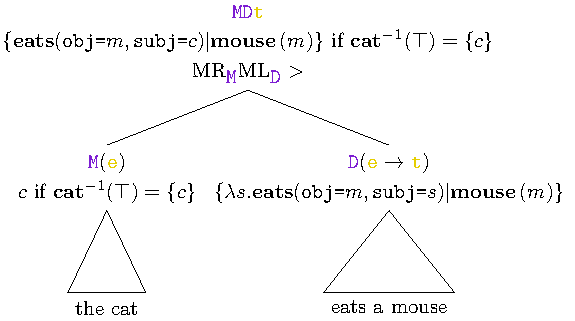
\includegraphics{aux/figures/parse-tree-2.pdf}
	\end{center}

	\centering
	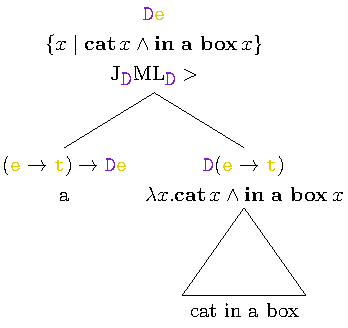
\includegraphics{aux/figures/parse-tree-1.pdf}

	\begin{center}
		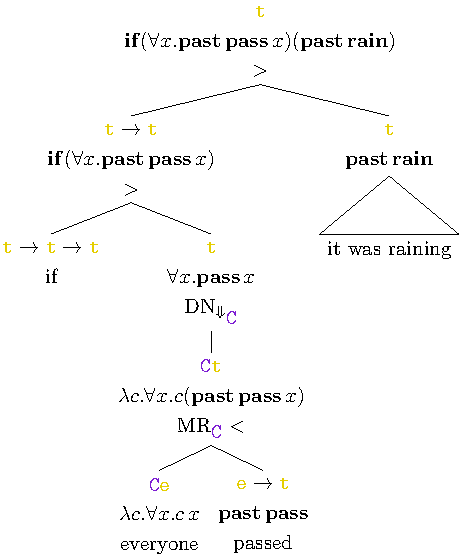
\includegraphics[height=.7\pageheight]{aux/figures/parse-tree-3.pdf}
	\end{center}
\end{frame}

\subsection{String diagrams for parsing}
\begin{frame}
	\frametitle{Combinators as String Diagrams}
	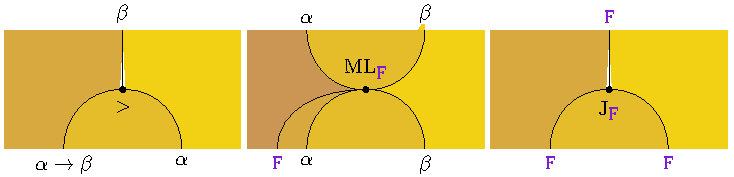
\includegraphics[width=\textwidth]{aux/figures/combinators-sd.pdf}
\end{frame}

\begin{frame}
	\frametitle{A Parsing Diagram Step}
	\centering
	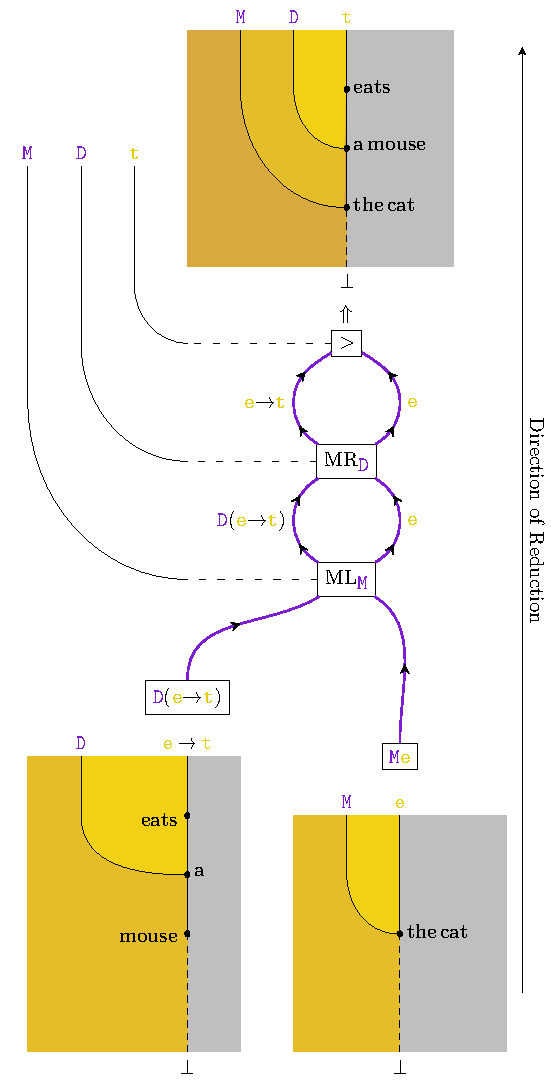
\includegraphics[height=.8\textheight]{aux/figures/parsing-diagram.pdf}
\end{frame}

\begin{frame}
	\frametitle{Another Parsing Diagram Step}
	\centering
	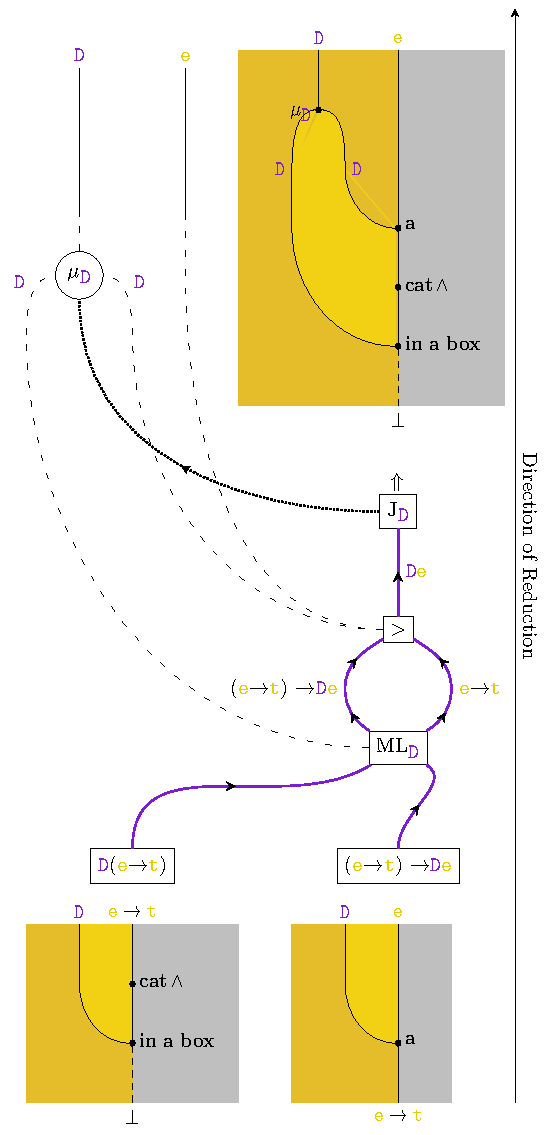
\includegraphics[height=.8\textheight]{aux/figures/parsing-diagram2.pdf}
\end{frame}

\begin{frame}
	\frametitle{Building an Intuition}
	\centering
	
\includegraphics[width=.7\textwidth]{aux/figures/knitting-example.jpeg}
\end{frame}

\begin{frame}
	\frametitle{A Full Parsing Diagram}
	\centering
	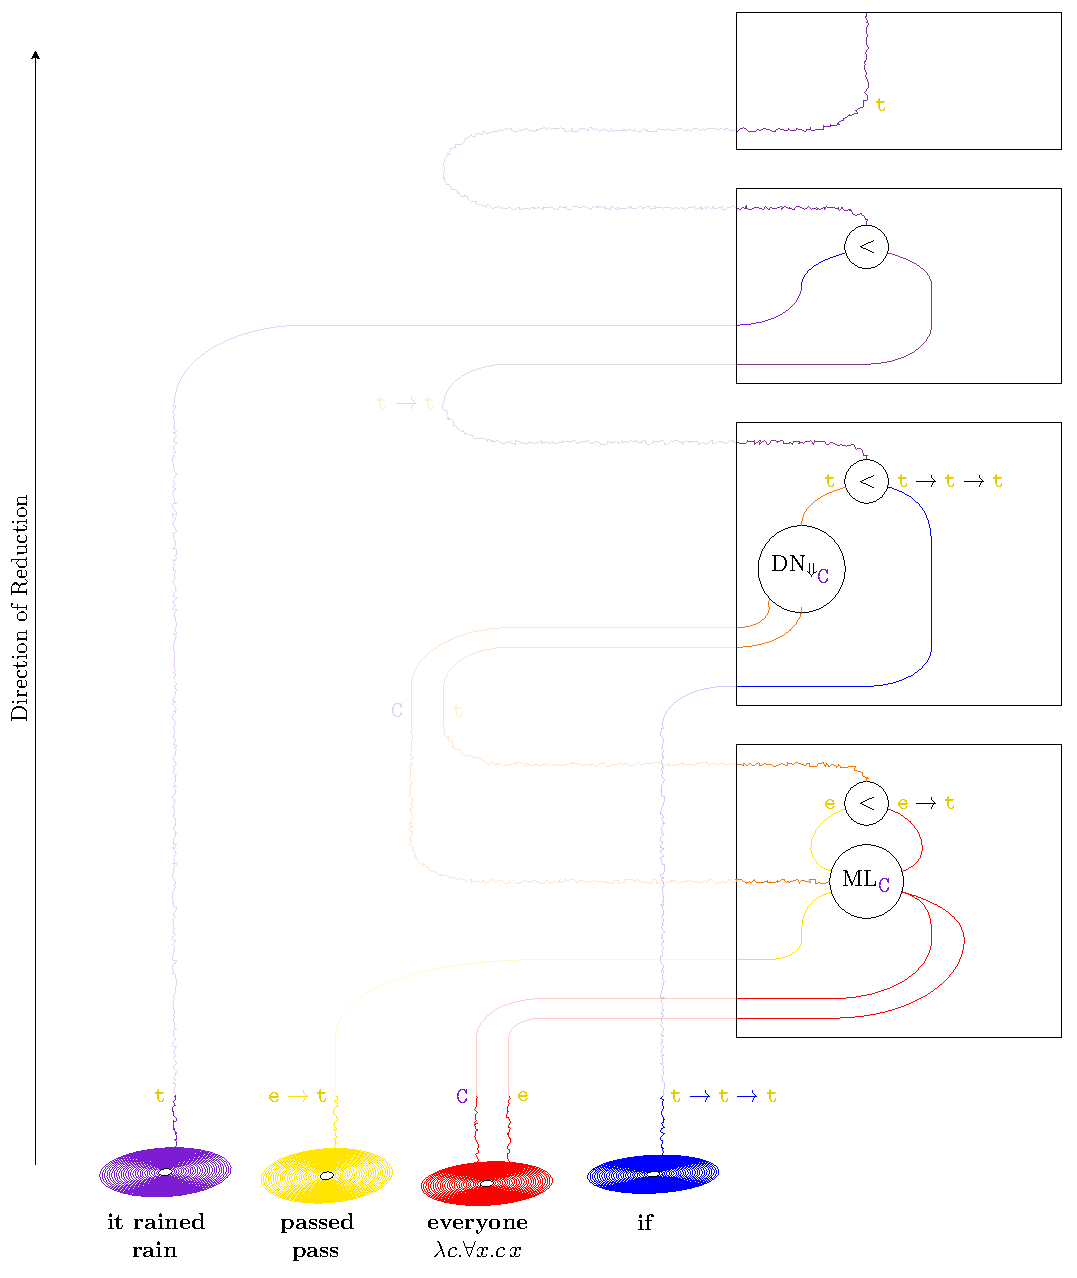
\includegraphics[height=.8\textheight]{aux/figures/3d-parsing-diagram.pdf}
\end{frame}

\subsection{String diagrams for reductions}
\begin{frame}
	\frametitle{Reducing the grammar}
	We translate equalities on actual denotations (from combinators or from the denotational system) into the reduction system on string diagrams.
	\smallskip

	Commutation of effects, Theorem \ref{thm:isotopy} and more, allow a reduction of the constant in the algorithmic complexity.
\end{frame}

\begin{frame}
	\frametitle{Conclusion}
	\begin{itemize}
		\item Theoretical enhancement of a type system for natural language semantics;
		      \pause
		\item No load added neither on the user (comprehension) nor the parser (efficiency).
	\end{itemize}

	\pause\medskip

	I would like to thank Simon Charlow for his advice and guidance, my mother for the
	knitting, Antoine Groudiev for the rotation of the snakes in equation labels,
	Bella Senturia, Bob Frank and Paul-André Melliès for their suggestions of
	papers to read about categories and linguistics.
\end{frame}

\appendix

\questionsframe
\begin{frame}
	\frametitle{Lexicon}
	\centering
	\adjustbox{height=.4\textheight}{	\setcellgapes{2pt}
	\makegapedcells
	\begin{NiceTabular}{>{\bf}LLL}
		Expression & \rm Type & \lambda\text{-Term} \\
		\word{planet}{\e\to\t}{\lambda x. \w{planet} x}{common nouns}
		\word{carnivorous}{\left( \e \to \t \right)}{\lambda x. \w{carnivorous}x}{predicative adjectives}
		\word{skillful}{\left( \e \to \t \right) \to \left( \e \to \t \right)}{\lambda p. \lambda x. px \land \w{skillful} x}{predicate modifier adjectives}
		\word{Jupiter}{\e}{{\bf j}\in \Var}{proper nouns}
		\word{sleep}{\e \to \t}{\lambda x. \w{sleep} x}{intranitive verbs}
		\word{chase}{\e \to \e \to \t}{\lambda o. \lambda s. \mathbf{chase}\left( o \right)\left( s \right)}{transitive verbs}
		\word{be}{\left( \e \to \t \right) \to \e \to \t}{\lambda p. \lambda x. px}{}
		\word{she}{\e\to\e}{\lambda x. x}{}
		\word{it}{\left( \bot \to \f{G}\e \right)}{\lambda g. g_{0}}{}
		\word{which}{\left( \e \to \t \right)\to \f{S}\e}{\lambda p. \left\{x \suchthat px\right\}}{}
		\word{the}{\left( \e \to \t \right) \to \f{M}\e}{\lambda p. x \text{ if } p^{-1}\left( \top \right) = \{x\} \text{ else } \#}{}
		\word{a}{\left( \e \to \t \right) \to \f{D}\e}{\lambda p. \lambda s. \left\{ \scalar{x, x + s}\suchthat p x\right\}}{}
		\word{no}{\left( \e \to \t \right) \to \f{C}\e}{\lambda p. \lambda c. \lnot \exists x. p x \land c\, x}{}
		\word{every}{\left( \e \to \t \right)\to \f{C}\e}{\lambda p. \lambda c. \forall x, px \Rightarrow cx}{}
		\CodeAfter
		\begin{tikzpicture}
			\draw[double] (1|-2) -- (4|-2);
			\foreach \r in {4,6,...,14} {\draw (1|-\r) -- (4|-\r);}
			\foreach \r in {15,...,21} {\draw (1|-\r) -- (4|-\r);}
		\end{tikzpicture}
	\end{NiceTabular}
}
\end{frame}

\begin{frame}
	\frametitle{Functor Denotations}
	\resizebox{\textwidth}{!}{	\def\arraystretch{1.3}
	\setcellgapes{2pt}
	\makegapedcells
	\begin{NiceTabular}{LLc}
		\rm Constructor                                              & \fmap                                                                                     & Typeclass \\
		\f{G}\left( \tau \right) = \r \to \tau                       & \f{G}\phi\left( x \right) = \lambda r. \phi \left(x r\right)                              & Monad     \\
		\f{W}\left( \tau \right) = \tau \times \t                    & \f{W}\phi\left( \left( a, p \right) \right) = \left( \phi a, p \right)                    & Monad     \\
		\f{S}\left( \tau \right) = \{ \tau \}                        & \f{S}\phi\left( \left\{ x \right\} \right) = \left\{ \phi(x) \right\}                     & Monad     \\
		\f{C}\left( \tau \right) = \left( \tau \to \t \right) \to \t & \f{C}\phi\left( x \right) = \lambda c. x\left( \lambda a. c \left( \phi a \right) \right) & Monad     \\
		\f{M}\left( \tau \right) = \tau + \bot                       & \f{M}\phi\left( x \right) = \begin{cases}
			                                                                                           \phi\left( x \right) & \text{if } \cont x: \tau \\
			                                                                                           \#                   & \text{if } \cont x: \#
		                                                                                           \end{cases}                                        & Monad                \\
		\CodeAfter
		\begin{tikzpicture}
			\draw[double] (1|-2) -- (5|-2);
			\foreach\r in {3,...,6} {%
					\draw (1|-\r) -- (5|-\r);
				}
		\end{tikzpicture}
	\end{NiceTabular}
}
\end{frame}

\begin{frame}
	\frametitle{CFG of English}
	\centering
	\small
	\begin{minipage}{.45\textwidth}
		\setlength\tabcolsep{4pt}
		\begin{tabular}{>{\tt}l r >{\tt}l r}
			\firstrule{CP}{DP, VP}{}
			\grule{Cmp, CP}{}
			\grule{CP, CBar}{}
			\gskip
			\firstrule{CBar}{Cor, CP}{}
			\gskip
			\firstrule{Dbar}{Cor, DP}{}
			\gskip
			\firstrule{DP}{DP, Dbar}{}
			\grule{Dmp, DP}{}
			\grule{Det, NP}{}
			\grule{Gen, TN}{}
			\gskip
			\firstrule{Gen}{DP, GenD}{}
		\end{tabular}
	\end{minipage}
	\begin{minipage}{.45\textwidth}
		\setlength\tabcolsep{4pt}
		\begin{tabular}{>{\tt}l r >{\tt}l r}
			\firstrule{NP}{AdjP, NP}{}
			\grule{NP, AdjP}{}
			\gskip
			\firstrule{AdjP}{TAdj, DP}{}
			\grule{Deg, AdjP}{}
			\gskip
			\firstrule{VP}{TV, DP}{}
			\grule{AV, CP}{}
			\grule{VP, AdvP}{}
			\gskip
			\firstrule{TV}{DV, DP}{}
			\gskip
			\firstrule{AdvP}{TAdv, DP}{}
		\end{tabular}
	\end{minipage}

\end{frame}

\begin{frame}
	\frametitle{CFG for Parsing}
	\begin{minipage}{.9\textwidth}
		\begin{multicols}{2}
			\def\arraystretch{1.1}
			\begin{mgrammar}
				\firstrule{>, \beta}{\left(\alpha\to \beta\right), \alpha}{}
				\firstrule{<, \beta}{\alpha, \left(\alpha \to \beta\right)}{}
				\gskip
				\firstrule{\combJ_{\f{F}}\  \f{F}\tau}{\f{F}\f{F}\tau}{}
				\firstrule{\combDN_{\f{C}}\  \tau}{\f{C}_{\tau}\tau}{}
				\gskip
				\firstrule{\combML_{\f{F}} \left(\alpha, \beta\right)}{\f{F}\alpha, \beta}{}
				\firstrule{\combMR_{\f{F}} \left(\alpha, \beta\right)}{\alpha, \f{F}\beta}{}
			\end{mgrammar}

			\def\arraystretch{1.3}
			\begin{mgrammar}
				\firstrule{\combA_{\f{F}} \left(\alpha, \beta\right)}{\f{F}\alpha, \f{F}\beta}{}
				\firstrule{\combUR_{\f{F}} \left(\alpha \to \alpha', \beta\right)}{\f{F}\alpha\to \alpha', \beta}{}
				\firstrule{\combUL_{\f{F}} \left(\alpha, \beta\to \beta'\right)}{\alpha, \f{F}\beta \to \beta'}{}
				\firstrule{\combC_{\f{L}\f{R}} \left(\f{L} \alpha, \f{R}\beta\right)}{\left(\alpha, \beta\right)}{}
				\firstrule{\combER_{\f{R}} \left(\f{R}\left(\alpha \to \alpha'\right), \beta\right)}{\alpha\to \f{R}\alpha', \beta}{}
				\firstrule{\combEL_{\f{R}} \left(\alpha, \f{R}\left(\beta \to \beta'\right)\right)}{\alpha, \beta\to \f{R}\beta'}{}
			\end{mgrammar}
		\end{multicols}
	\end{minipage}

\end{frame}

\begin{frame}
	\frametitle{Combinator Denotations}
	\scriptsize
	\centering
	$	>                    = \lambda \phi. \lambda x. \phi x $\\[1.5ex]
	$ <                    = \lambda x. \lambda \phi. \phi x $\\[1.5ex]
	$ \combML_{\f{F}}      = \lambda M. \lambda x. \lambda y. (\fmap_{\f{F}} \lambda a. M(a, y)) x $\\[1.5ex]
	$ \combMR_{\f{F}}      = \lambda M. \lambda x. \lambda y. (\fmap_{\f{F}} \lambda b. M(x, b)) y $\\[1.5ex]
	$	\combA_{\f{F}}       = \lambda M. \lambda x. \lambda y. (\fmap_{\f{F}}\lambda a. \lambda b. M(a, b))(x) \texttt{<*>} y $\\[1.5ex]
	$	\combUL_{\f{F}}      = \lambda M. \lambda x. \lambda \phi. M(x, \lambda b. \phi(\eta_{\f{F}} b))$\\[1.5ex]
	$	\combUR_{\f{F}}      = \lambda M. \lambda \phi. \lambda y. M(\lambda a. \phi(\eta_{\f{F}} a),y) $\\[1.5ex]
	$ \combJ_{\f{F}}       = \lambda M. \lambda x. \lambda y. \mu_{\f{F}} M(x, y) $\\[1.5ex]
	$\combC_{\f{L}\f{R}}  = \lambda M. \lambda x. \lambda y. \epsilon_{\f{L}\f{R}}(\fmap_{\f{L}}(\lambda l. \fmap_{\f{R}}(\lambda r. M(l, r))(y)) (x))$\\[1.5ex]
	$	\combEL_{\f{R}}      = \lambda M. \lambda \phi. \lambda y. M(\Upsilon_{\f{R}} \phi, y)$\\[1.5ex]
	$	\combER_{\f{R}}      = \lambda M. \lambda x. \lambda \phi. M(x, \Upsilon_{\f{R}} \phi)$\\[1.5ex]
	$	\combDN_{\Downarrow} = \lambda M. \lambda x. \lambda y. \Downarrow M(x, y)$
\end{frame}

\begin{frame}[allowframebreaks]
	\frametitle{Bibliography}
	\printbibliography
\end{frame}

\end{document}

